\documentclass{article}
\usepackage{ctex}
\usepackage{makecell}
\usepackage{graphicx}
\usepackage{geometry}
\usepackage{multirow}
\usepackage{multicol}
\usepackage{fancyhdr}
\usepackage{longtable}
\usepackage{color}
\usepackage{float}
\usepackage{listings}
\usepackage{xcolor}
\usepackage{hyperref}
\usepackage{footnote}
\usepackage{paralist}
\usepackage{amsmath}
\usepackage{subcaption}

\let\itemize\compactitem
\let\enditemize\endcompactitem
\let\enumerate\compactenum
\let\endenumerate\endcompactenum
\let\description\compactdesc
\let\enddescription\endcompactdesc

\geometry{a4paper,left=25mm,right=20mm,top=25mm,bottom=25mm}

\title{数字图像处理实验三}
\author{09021227~金桥}
\date{\today}

\lstset{
    numbers=left,
    keywordstyle= \color{ blue!70},
    commentstyle= \color{red!50!green!50!blue!50},
    rulesepcolor= \color{ red!20!green!20!blue!20} ,
    % escapeinside=``,
    numberstyle=\tt,
    numbersep=0em,
    xleftmargin=2em,
    breaklines,
    aboveskip=1em,
    framexleftmargin=2em,
    frame=shadowbox,
    basicstyle=\tt,
    language=C++
}

\begin{document}

\maketitle

\section{实验目标}

PPT 151页的月亮图像分别进行基于二阶导数 (建议用卷积操作完成)、非锐化掩蔽(Unsharp Masking) (分析不同参数的选择对结果的影响)两种方法的图像增强。

\section{过程与方法}

请注意,以下算法均为自主手动实现,\textbf{没有调用OpenCV的方法。}

\subsection{基于二阶导数的图像增强}

根据公式 $$\nabla^2f(x, y)=f(x+1, y)+f(x-1, y)+f(x, y+1)+f(x, y-1)-4f(x, y).$$ 有如下卷积核:
$$
\mathbf{w}=\left[
    \begin{matrix}
        0 & 1 & 0\\
        1 & -4 & 1\\
        0 & 1 & 0
    \end{matrix}
\right]
$$
设原图像为$f$, 则卷积后的图像为$\nabla^2f$, 最终得到的图像为$g$ 则有$$g=f+c\nabla^2f.$$ 其中$c$为参数。

\subsection{非锐化掩蔽}

这里采用了高斯模糊进行钝化。采用以下卷积核进行高斯模糊:
$$
\mathbf{w}=\left[
    \begin{matrix}
        0.094741 & 0.118318 & 0.094741\\
        0.118318 & 0.147761 & 0.118318\\
        0.094741 & 0.118318 & 0.094741
    \end{matrix}
\right]
$$
将原图像与卷积核进行卷积即可得到高斯模糊后的图像。

设原图像为$f$, 模糊后的图像为$\overline{f}$, 最终得到的图像为$g$ 则有$$g=f+k(f-\overline{f}).$$ 其中$k$为参数。

\section{结果与分析}

\subsection{基于二阶导数的图像增强}

下图为采用基于二阶导数的图像增强后的对比图。

\begin{figure}[H]
    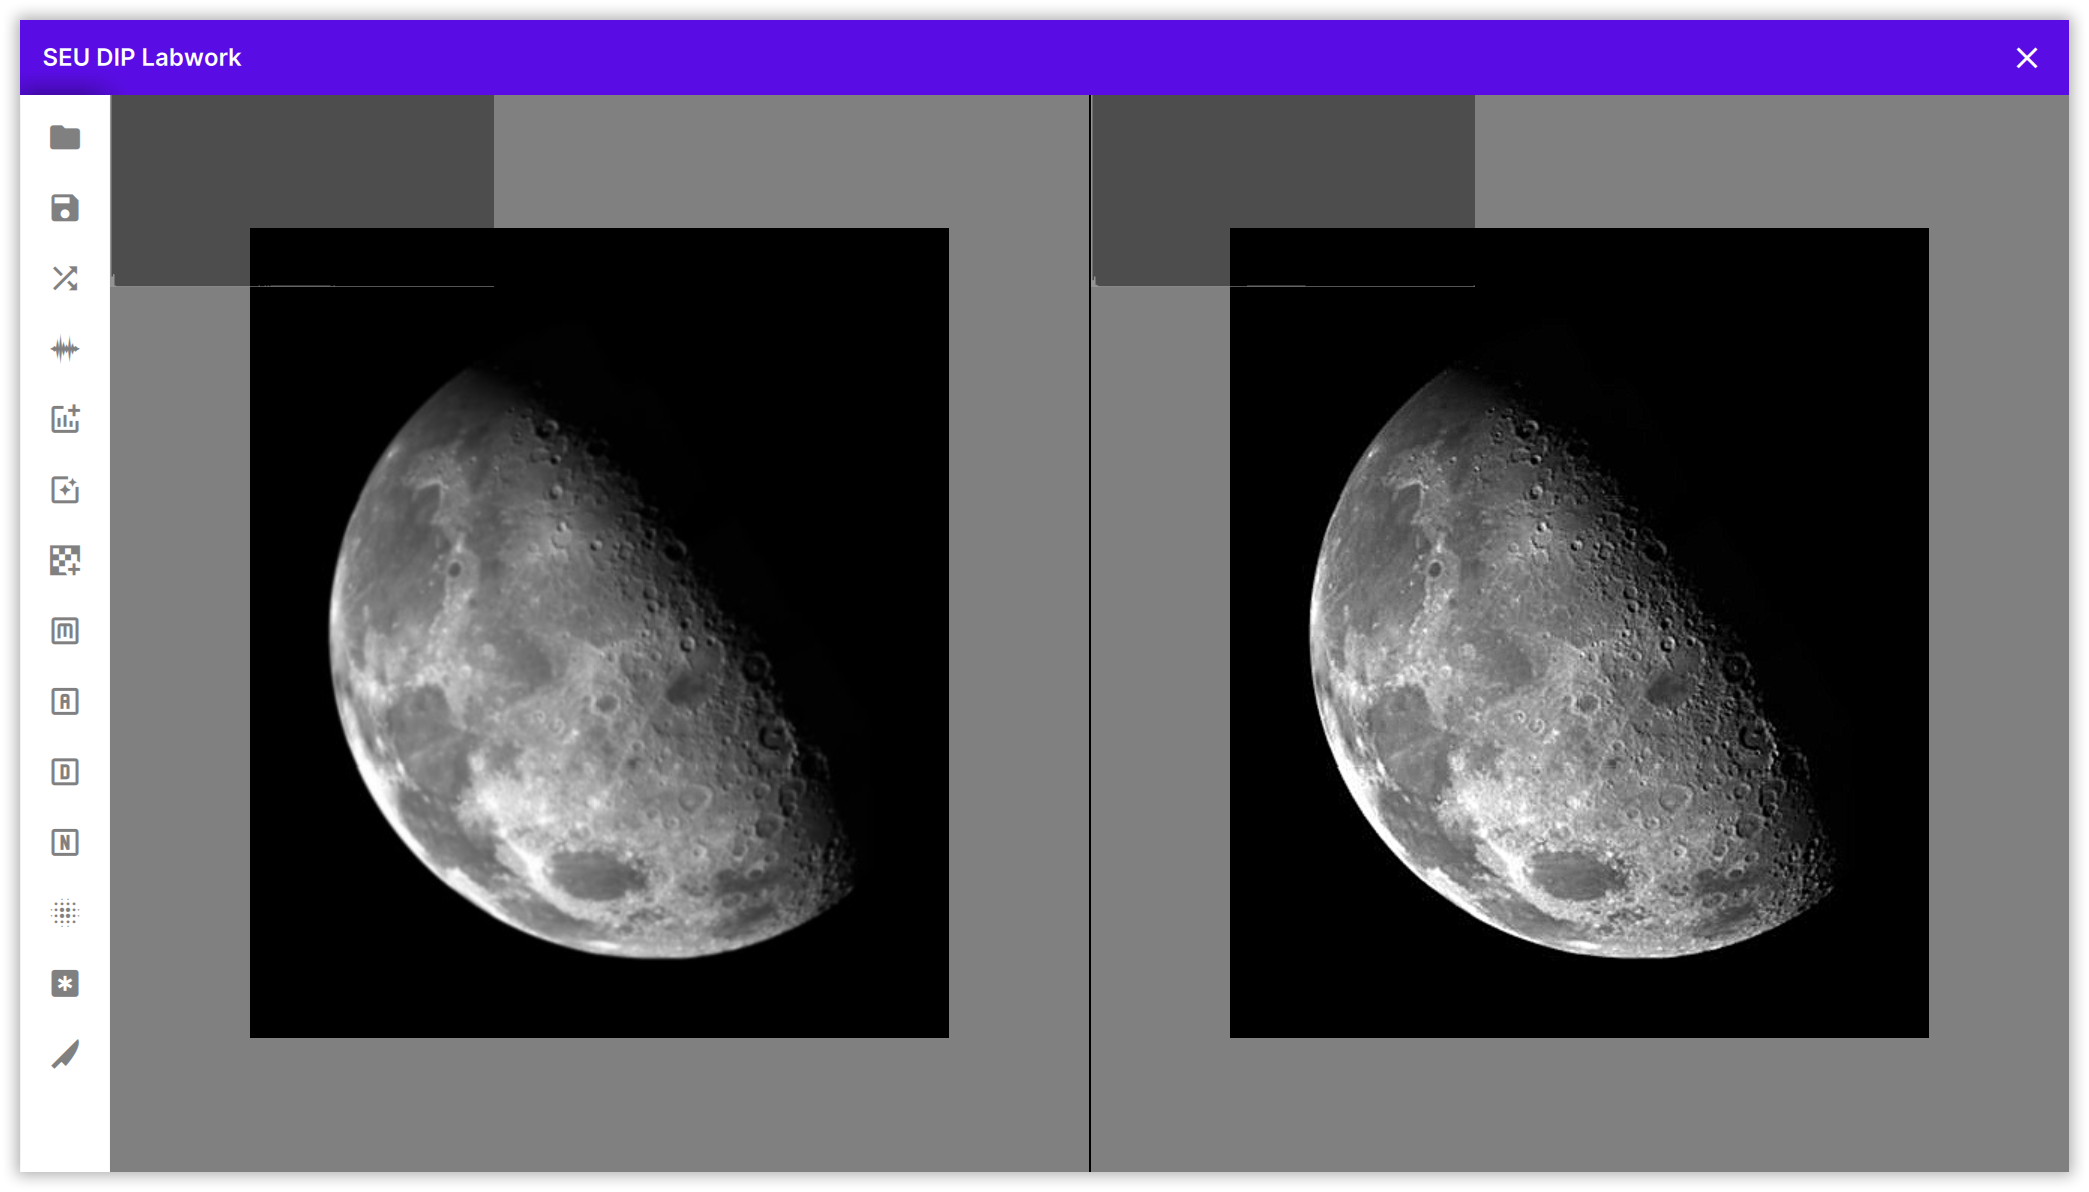
\includegraphics[width=\textwidth]{img/laplace-sharpening.png}
    \caption{左侧为原图像,右侧是经过锐化的图像}
\end{figure}

下图是基于二阶导数的图像增强调节参数$c$得到的图像(为了节省空间没有截取程序界面),从左到右分别是$c=-1, -2, -3$的结果。可以看到,随着$c$的增大,图像锐化程度也逐渐增加。

\begin{figure}[htbp]
    \centering
    \begin{subfigure}{.32\textwidth}
        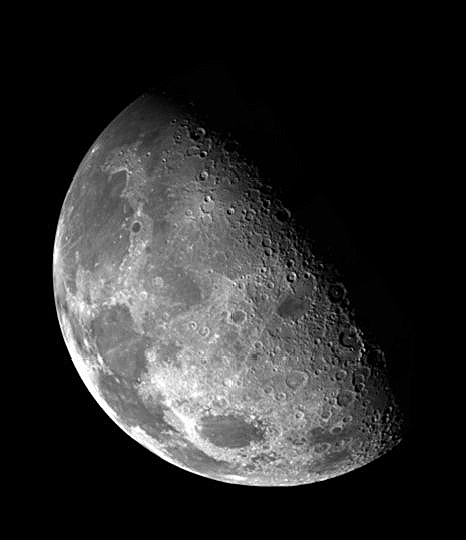
\includegraphics[width=\linewidth]{img/laplace/1.png}
        % \caption{Caption 1}
    \end{subfigure}
    \begin{subfigure}{.32\textwidth}
        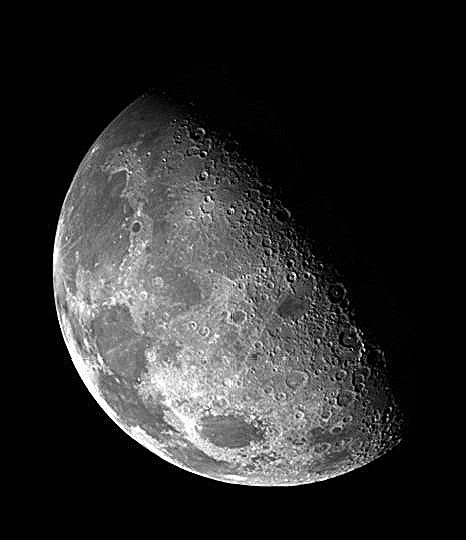
\includegraphics[width=\linewidth]{img/laplace/2.png}
        % \caption{Caption 2}
    \end{subfigure}
    \begin{subfigure}{.32\textwidth}
        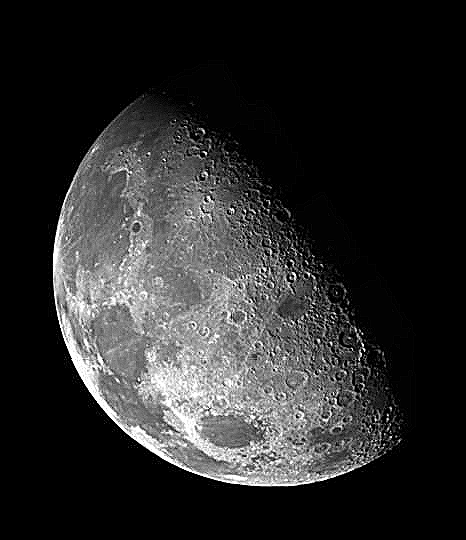
\includegraphics[width=\linewidth]{img/laplace/3.png}
        % \caption{Caption 3}
    \end{subfigure}
    \caption{从左到右分别是$c=-1, -2, -3$的结果}
\end{figure}

\newpage

\subsection{非锐化掩蔽}

下图为采用非锐化掩蔽后的对比图。

\begin{figure}[H]
    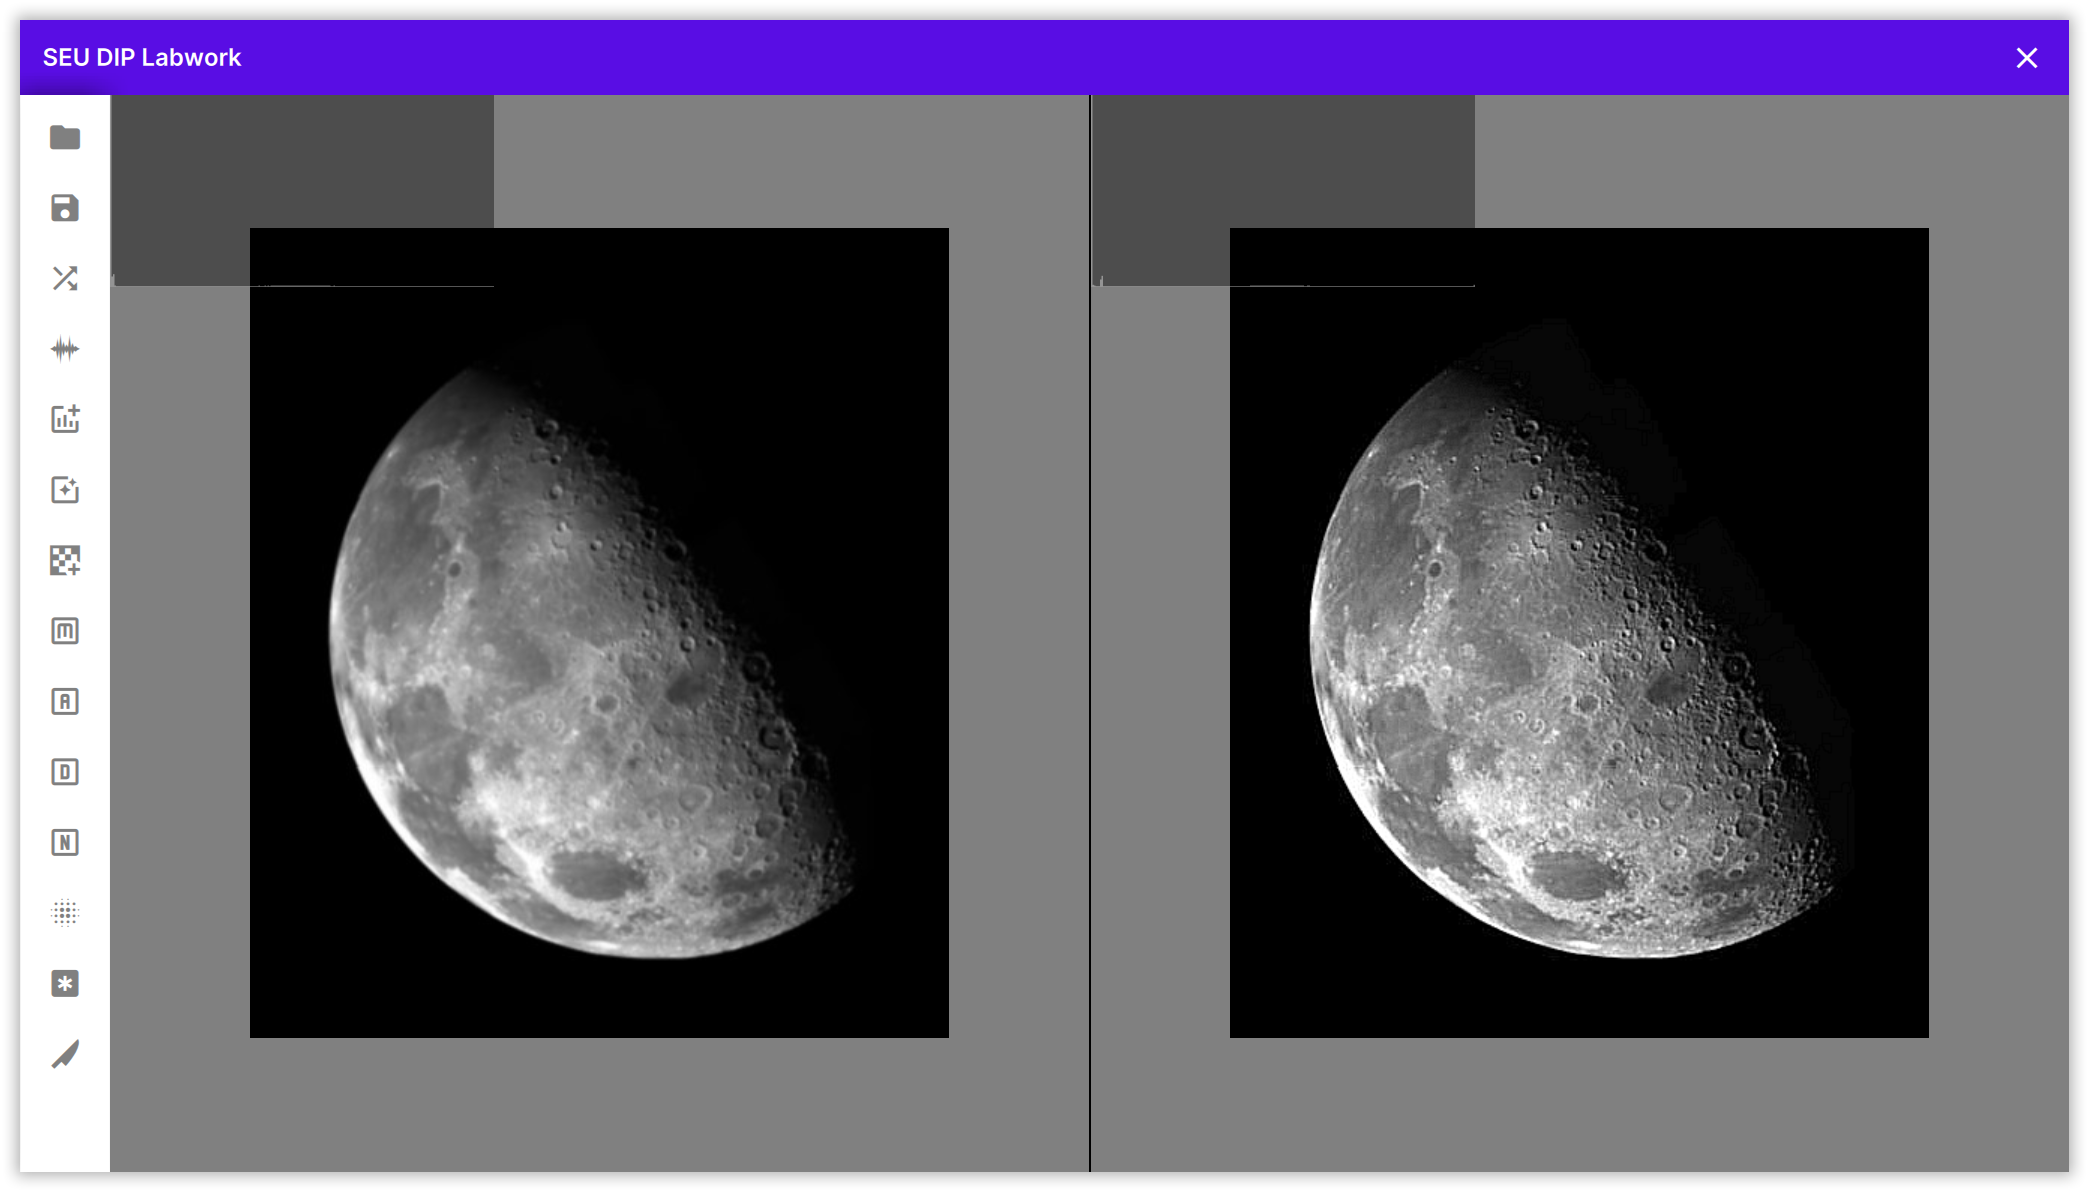
\includegraphics[width=\textwidth]{img/usm.png}
    \caption{左侧为原图像,右侧是经过锐化的图像}
\end{figure}

下图是非锐化掩蔽调节参数$k$得到的图像(为了节省空间没有截取程序界面),从左到右分别是$k=1, 5, 10$的结果。可以看到,随着$k$的增大,图像锐化程度也逐渐增加。

\begin{figure}[htbp]
    \centering
    \begin{subfigure}{.32\textwidth}
        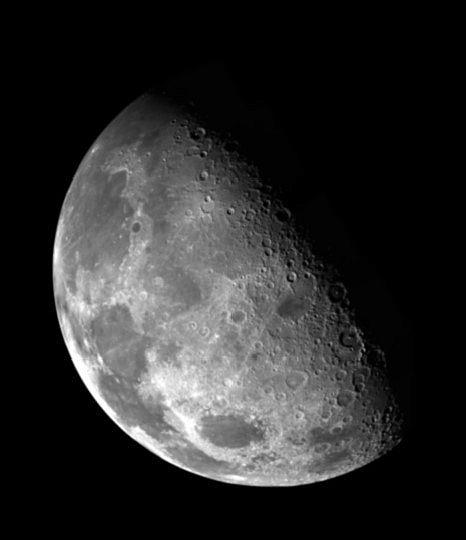
\includegraphics[width=\linewidth]{img/usm/1.png}
        % \caption{Caption 1}
    \end{subfigure}
    \begin{subfigure}{.32\textwidth}
        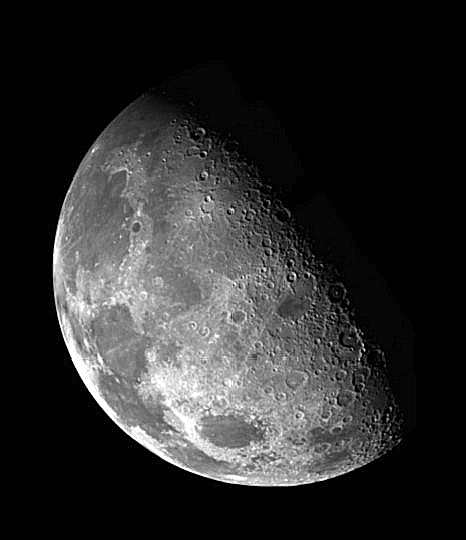
\includegraphics[width=\linewidth]{img/usm/5.png}
        % \caption{Caption 2}
    \end{subfigure}
    \begin{subfigure}{.32\textwidth}
        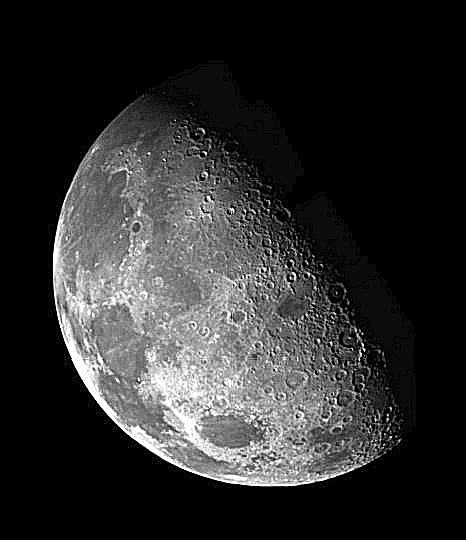
\includegraphics[width=\linewidth]{img/usm/10.png}
        % \caption{Caption 3}
    \end{subfigure}
    \caption{从左到右分别是$k=1, 5, 10$的结果}
\end{figure}

\end{document}
